% This work is licensed under the Creative Commons Attribution-NonCommercial 4.0 International License.
% To view a copy of this license, visit http://creativecommons.org/licenses/by-nc/4.0/
% or send a letter to Creative Commons, PO Box 1866, Mountain View, CA 94042, USA.

% !TEX TS-program = xelatex

\documentclass[../Main/chem371-notes.tex]{subfiles}

\setcounter{chapter}{6}
\begin{document}

\chapter{Density Functional Theory}

In the previous chapters, we discussed the Hartree--Fock method.
This approximation is insufficient to make accurate predictions of molecular properties because it neglects \emph{electron correlation} effects.
There are two main ways to include correlation effects in quantum chemistry computations: 1) density functional theory and 2) correlated wave function methods.
In this chapter we will discuss density functional theory (DFT), an approach that in the past several decades has revolutionized the field of quantum chemistry.
DFT is an approximate method, but in many cases it yields results of sufficient accuracy to make reliable predictions.

\section{Going beyond Hartree--Fock theory: Electron correlation}

\mfigure{\\
\centering{
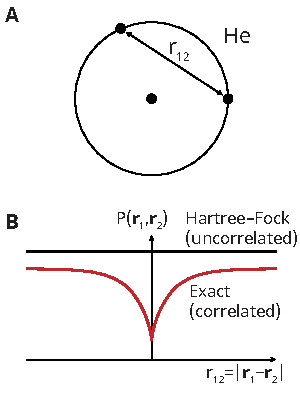
\includegraphics[width=1.75in]{img/correlation.pdf}
}
\captionof{figure}{Two electrons in the helium atom at equal distance from the nucleus (\textbf{A}). The probability of finding two electrons [$P(\mathbf{r}_1,\mathbf{r}_2)$] at a given radius as a function of their distance $r_{12}$ (\textbf{B}). }
\label{fig:dft:correlation}
}

From a classical point of view, electrons experience Coulomb repulsion, and consequently one would expect that their motion is influenced by their mutual interactions.
From a probabilist point of view, this means that it is more likely that two electrons are found at a large distance than at a shorter one.
In this case we say that the probability distribution of the electrons is \emph{correlated}.
From the point of view of quantum mechanics, this means that the probability of finding the electrons in positions/spin equal to $x_1, x_2, \ldots$, which we indicate with $P(x_1,x_2, \ldots)$, cannot be written as a product of individual electron probabilities
\begin{equation}
P(x_1,x_2, \ldots) = |\Psi(x_1,x_2, \ldots)|^2
\neq P_1(x_1) P_2(x_2) \cdots
\end{equation}

The Hartree--Fock method does fully account for electron correlation.\mnote{Hartree--Fock theory includes a special type of correlation for electrons with same spin, called Fermi correlation.}
This can be seen in Fig.~\ref{fig:dft:correlation}, where if we plot the probability of finding the electrons in the helium atom as a function of their distance--- while keeping their distance from the nucleus fixed---we find out that the Hartree--Fock wave function is a constant.
This is because for the case of Hartree--Fock the probability of finding the two electrons is the product of two independent probabilities.
Figure~\ref{fig:dft:correlation} also shows the exact wave function, which displays a dip in the probability due to Coulomb repulsion.

When doing quantum chemistry computations, we are mostly concerned with the effects of electron correlation on the energy. Therefore, we define the electron correlation energy ($E_\mathrm{corr}$) as the difference between the exact and the Hartree--Fock energies
\begin{equation}
E_\mathrm{corr} = E_\mathrm{exact} - E_\mathrm{HF}
\end{equation}
Because of the variational principle, the \emph{correlation energy is always negative}.

\section{Theoretical foundations of density functional theory}
One of the simplest way to include the effects of electron correlation is via density functional theory (DFT).
The basic idea of DFT is to avoid solving the $N$-electron Schr\"{o}dinger equation, which requires us to determine the wave function $\Psi(x_1,x_2, \ldots)$.
Instead, DFT tries to capture the properties of the ground state only using the \emph{electron density} $\rho(x)$.
This quantity is derived from the full electron wave function by squaring and integrating over all particle coordinates except for the first coordinate ($x_1$)
\begin{equation}
\rho(x_1) = N \int dx_2 \, dx_3 \ldots |\Psi(x_1,x_2, \ldots)|^2
\end{equation}
Since $\rho(x_1)$ is a function of 3 spatial coordinates and one spin coordinate, it is much easier to represent and compute.

\mfigure{\\
\centering{
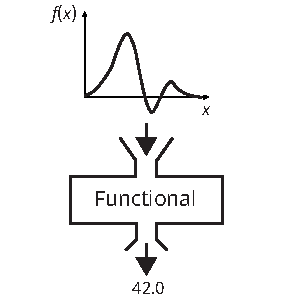
\includegraphics[width=1.75in]{img/functional.pdf}
}
\captionof{figure}{A functional is a mathematical operation that converts a function, $f(x)$, into a number. }
\label{fig:dft:functional}
}

DFT was put on solid theoretical grounds by the work of Hohenberg and Kohn (1964).
These authors established the existence of a universal \emph{functional} of the density $E[\rho]$, such that the energy of the ground state can be obtained by minimizing $E[\rho]$ with respect to the density
\begin{equation}
\min_\rho E[\rho] = E_\mathrm{exact}
\end{equation}
As shown in Fig.~\ref{fig:dft:functional}, functional $F[f]$ is a mathematical operation that converts a function $f(x)$ into a number
\begin{equation}
F : F[f(x)] \rightarrow \mathbb{R}
\end{equation}
In many cases functionals are integrals of the input function.
The following two examples are functionals that convert $f$ to a number
\begin{equation}
F[f(x)] = \int dx \, |f(x)|^2,\quad F[f(x)] = \int dx_1 dx_2 \, \frac{f(x_1) f(x_2)}{|x_1 - x_2|},
\end{equation}

Going back to DFT, the density $\rho(x)$ that minimizes the functional $E[\rho]$ corresponds to the exact ground state density ($\rho_\mathrm{exact}$).
Unfortunately, the work of Hohenberg and Kohn only proved the existence of the exact functional.
\emph{The exact form of this functional is unknown}, at it is likely that we may not be able to write it down in a closed form.

A second important development was the introduction of the \emph{Kohn--Sham method}, which is a practical way to apply DFT theory.
The Kohn--Sham method is so fundamental that it has now become a synonym for density functional theory, and any computational code that implements DFT is basically performing a computation with the Kohn--Sham method.
In the Kohn--Sham method, we reintroduce orbitals with the purpose of obtaining a better numerical approximation to the energy.
Once we know the orbitals, the density can be obtained as a sum of the orbital squared (you can think of this as adding up the probability distribution for each electron)
\begin{equation}
\rho(x_1) = \sum_i^{\mathrm{electrons}} |\psi_i(x_1)|^2
\end{equation}
The KS DFT functional is then a functional of the orbitals ($E_\mathrm{KS} [\{\psi_i\}]$) and the density and contains four contributions
\begin{equation}
\label{eq:dft:ksenergy}
E_\mathrm{KS} [\{\psi_i\}] = T[\{\psi_i\}] + V_\mathrm{en}[\rho] + J[\rho] + E_\mathrm{xc}[\rho]
\end{equation}
These terms represent four different contributions to the energy
\begin{myitems}
\item $T[\{\psi_i\}]$: The kinetic energy functional. This function is known exactly and it uses information from the orbitals to compute the kinetic energy.
\item $V_\mathrm{en}[\rho]$: The electron-nucleus interaction energy. This terms accounts for the Coulomb interaction of the negative electron charge with the positive charge of the nuclei. This energy contributions is given by a functional that is known exactly and it depends only on the electron density.
\item $J[\rho]$: The Coulomb functional. This function takes in to account the classical Coulomb interaction of the electron density with itself.
\item $E_\mathrm{xc}[\rho]$: The exchange-correlation (xc) functional. This is the part of the functional that accounts for exchange and correlation effects. With exchange, we mean corrections to the energy due to the fact that the wave function must be antisymmetric (exchange terms are already included in Hartree--Fock theory). We add exchange because this is a purely quantum mechanical contributions that is not contained in $J[\rho]$.
With correlation, we instead mean all corrections to the energy due to the fact that electrons avoid each other due to Coulomb repulsion. In practice, this is the place where we push all the contributions to the energy that we do not exactly how to model.
\end{myitems}

\section{A practical guide to density functionals}

Because the exact exchange-correlation functional is unknown, practical implementations of DFT have to use approximate mathematical functionals that are optimized by fitting DFT results to experimental or theoretical results.
Typically, density functionals are a combination of many terms.
The exchange-correlation functional is divided into two separate terms that account for exchange and correlation separately
\begin{equation}
E_\mathrm{xc}[\rho] = E_\mathrm{x}[\rho] + E_\mathrm{c}[\rho]
\end{equation}

The simplest form of density functionals is the \emph{local density approximation} (LDA).
LDA functionals only depend on the density and example is the Dirac exchange functional
\begin{equation}
E_\mathrm{x}^\mathrm{Dirac} = - C_\mathrm{x} \int dx [\rho(x)]^{4/3}
\end{equation}

LDA functionals consider only the density at one point and can describe well systems with a homogeneous electron density.
However, they tend to perform poorly for molecules because the density of molecules is far from being homogeneous!
One way to go beyond LDA is the \emph{generalized gradient approximation} (GGA).
GGA functionals depend both on the density $\rho(x)$ and its gradient $\nabla \rho(x)$.
The gradient term helps improve the quality of the DFT functional by keeping into account the fact that $\rho(x)$ is not homogeneous.
For example, Becke's GGA exchange functional is given by
\begin{equation}
E_\mathrm{x}^\mathrm{B88} = - \beta \int dx [\rho(x)]^{4/3} \frac{|\nabla \rho(x)|}{\rho(x)} \frac{1}{1 + 6 \beta \sinh^{-1} (|\nabla \rho(x)|/\rho(x))}
\end{equation}
where $\beta$ is a parameter.
There are several commonly used GGA functionals, including BLYP, PBE, 

A significant improvement in the performance of GGA can be obtained by adding a small fraction of the exchange contribution from Hartree--Fock theory.
This family of functionals is called \emph{hybrids} and it is computationally more expensive than regular GGAs.
The most popular among the GGA functionals is \emph{Becke's 3-parameter functional (B3LYP)}, which is defined as
\begin{equation}
{\displaystyle E_{\text{xc}}^{\text{B3LYP}}=E_{\text{x}}^{\text{LDA}}+a_{0}(E_{\text{x}}^{\text{HF}}-E_{\text{x}}^{\text{LDA}})+a_{\text{x}}(E_{\text{x}}^{\text{GGA}}-E_{\text{x}}^{\text{LDA}})+E_{\text{c}}^{\text{LDA}}+a_{\text{c}}(E_{\text{c}}^{\text{GGA}}-E_{\text{c}}^{\text{LDA}}),}
\end{equation}
This functional mixes exchange and correlation functions from the LDA and GGA, and contains a contribution (20\%) from Hartree--Fock exchange $E_{\text{x}}^{\text{HF}}$.
Another common type of functional is PBE0, which mixes the PBE functional with Hartree--Fock exchange (25\%).

Another way to improve the performance of GGA functionals is to add terms that depend on the second derivatives of the density.
This choice leads to \emph{meta-GGA} functionals, which contain terms proportional to $\nabla^2 \rho(x)$.
Examples of meta-GGA include the TPSS functional, the Minnesota family of functionals (M05-L, M06-L, \ldots), and the B97M-V functional.
meta-GGA functionals can be combined with Hartree--Fock exchange to give hybrid meta-GGAs (like M06).

%\subsection{Range-separated hybrid functionals}
One last class of functionals are \emph{range-separated hybrid} functionals like ωB97M-V.
In these functionals, the amount of Hartree--Fock exchange included in the functional depends on the distance between electrons ($r_{12}$).
At short distances, these functionals use less than 100\% of HF exchange, while they include the full amount at infinite electron separation.
This splitting separate the exchange energy into a short-range (SR) plus a long-range (LR) term
\begin{equation}
E_\mathrm{x} = E_\mathrm{x}^\mathrm{SR} + E_\mathrm{x}^\mathrm{LR}\end{equation}
Range-separated functionals play an important role in excited-state extensions of DFT (time-dependent DFT, TDDFT) and provide greater flexibility in the optimization of functionals.


\section{Limitations of approximate DFT functionals}

Despite significant efforts to optimize approximated density functionals, the functionals currently available cannot be applied across all problems in chemistry.
A recent review by Mardirossian and Head--Gordon [\textit{Mol. Phys.}, \textbf{115}, 2315 (2017)] summarizes the current status of DFT in the following way
\begin{quote}
Despite the `systematic' improvement offered by additional physical ingredients, there are three major limitations to the exchange-correlation functionals described above that cannot be remedied by the inclusion of local ingredients such as $\rho$, $\nabla \rho$, and $\nabla^2 \rho$: (1) self-interaction error (SIE), (2) long-range dynamic correlation (dispersion), and (3) strong correlation.
%
%Ultimately, today's state-of-the-art functionals are close to achieving the level of accuracy desired for a broad range of chemical applications, and the principal remaining limitations are associated with systems that exhibit significant self-interaction/delocalisation errors and/or strong correlation effects.
\end{quote}

The \emph{self-interaction error} (SIE) is an artifact of approximate density functionals and leads to incorrect energies even for systems containing one electron. 
For one-electron systems, there is no electron-electron interaction energy and in an exact functional the last two terms of Eq.~\eqref{eq:dft:ksenergy} should cancel out, that is $J[\rho] + E_\mathrm{xc}[\rho] = 0$.
Note that in Hartree--Fock theory the electron-electron interaction energy can be written as
\begin{equation}
J[\rho] + E_\mathrm{x}^\mathrm{HF}[\rho],
\end{equation}
and \emph{this term is identically zero for one-electron systems} (in other words, Hartree--Fock theory is exact for all one-electron systems).
To provide an example of the SIE, we will consider the energy of the hydrogen atom.
Using the cc-pV6Z basis set, the Hartree--Fock method gives an energy equal to $-$0.499999 \Eh, which is nearly converged to the exact energy $-$0.5 \Eh.
BLYP (a GGA functional) yields a higher energy ($-$0.497908 \Eh), while B3LYP (a hybrid GGA) gives an energy that falls below the exact value ($-$0.502440 \Eh).
Range separated functionals are also not immune to the SIE, with the ωB97M-V functional giving and error even larger than BLYP ($-$0.494675 \Eh).
Therefore, hybrid density functionals that include a fraction of HF exchange suffer less from the SIE.
Range-separated functionals are also less susceptible to the SIE error.
Another way to illustrate the SIE is by considering the \ce{H2+} molecule.
At infinite distance, the energy of \ce{H2+} should be identical of that of a H atom ($-$0.5 \Eh) plus a \ce{H+} ion (0 \Eh).
Instead energies from approximate density functionals for \ce{H2+} with a 100 \AA{} H-H distance are $-$0.606551 \Eh for BLYP, $-$0.587652 \Eh for B3LYP, and $-$0.534163 \Eh for ωB97M-V.
These values deviate significantly from the exact value due to the SIE.

\emph{Dispersion corrections} are another important recent development in DFT.
Dispersion forces (also known as London or van der Waals forces) arise from long-range correlation of electrons.
Energy corrections due to dispersion interactions are quite weak, and they rapidly decay as $R^{-6}$, where $R$ is the distance between two atoms.
Due to the long-range nature of dispersion interactions, density functionals that employ only local information about the density (its value and first few derivatives) have difficulties capturing this effect.
Neglecting the dispersion energy can introduce some important errors.
For example, 

A pragmatic way to introduce dispersion corrections in DFT has been to add the classical dispersion interaction of atoms to DFT computations.
For example, in the D$n$ corrections by Grimme and co-workers, the Kohn--Sham functional is augmented with a classical interaction term between atoms that contains terms proportional to $R_{ij}^{-6}$ and $R_{ij}^{-8}$, where $R_{ij}$ is the distance between atoms $i$ and $j$.
Because these terms diverge when $R_{ij}$ approaches zero, the dispersion energy is damped with a function that depends on $R_{ij}$.
The B3LYP-D3 approach is now considered an important alternative to B3LYP and is a good starting point if you want to describe systems that contain important contributions from long-range dispersion interactions.
Some examples of such systems include two non-bonded fragments, the interaction of bulky aliphatic groups, and interactions involving aromatic rings.

Another alternative is to use a density functional that can account for dispersion interactions.
Such functionals are called \emph{nonlocal} because the potential experienced by the electrons is modified by a term that depends on the density at a far distance.
The range-separated ωB97M-V functional accounts for dispersion interactions via the VV10 functional by Vydrov and Van Voorhis.

The problem of \emph{strong correlation} arises when considering bond-breaking processes and open-shell species with near-degenerate partially occupied orbitals.
The simplest example is the dissociation curve of \ce{H2}.
Approximate DFT methods predict a dissociation energy of \ce{H2} that is too large.
Strong correlation is an advanced topic and will considered more in detail in a later chapter of these notes.

\section{The cost of DFT and practical aspects}

The \emph{cost} of DFT computations is affected by several factors.
For a basis set containing $K$ elements, most vanilla implementations of DFT for quantum chemistry have a cost that scales as $K^4$.
A common technique to increase the speed of DFT is via \emph{density fitting} (DF) (also known as the resolution of the identity) or Cholesky decomposition.
Density fitting is an method to approximate the \emph{two-electron integrals} $(\varphi_i \varphi_j | \varphi_k \varphi_l)$ that enter in DFT (and Hartree--Fock) theory.
These integrals are defined as
\begin{equation}
(\varphi_i \varphi_j | \varphi_k \varphi_l) = 
\int d\mathbf{r}_1 \, d\mathbf{r}_2 \, \frac{\varphi^*_i(\mathbf{r}_1) \varphi_j(\mathbf{r}_1) \varphi^*_k(\mathbf{r}_2) \varphi_l(\mathbf{r}_2)}{r_{12}}
\end{equation}
There are $K^4$ of these type of integrals, because for each index ($i$, $j$, $k$, $l$) we can choose the orbital in $K$ different ways.
In density fitting, these two-electron integrals are approximated as the product of quantities that depend only on three indices ($L_{ij}^{Q}$)
\begin{equation}
(\varphi_i \varphi_j | \varphi_k \varphi_l) = \sum_Q^M L_{ij}^{Q} L_{kl}^{Q}
\end{equation}
To compute the quantities $L_{ij}^{Q}$, density fitting uses an \emph{auxiliary basis set}.
Therefore, to use density fitting you must also specify an auxiliary basis set.
For many families of basis sets (cc-pV$X$Z and Karlsruhe) there are corresponding auxiliary basis sets (usually they have the same name, but they carry the suffix -JK).
Typically the size of the auxiliary basis set is about 3 times larger than a conventional basis set.
The main advantage of density fitting is to reduce the cost of DFT computations that employ local functionals from $K^4$ to $K^3$.
Density fitting also reduces the cost of  hybrid functionals because it lowers the memory and disk storage requirements (since only about 3$K^3$ integrals have to be computed and stored).

In addition to selecting a basis set, DFT computations require choosing an \emph{integration grid}.
Integration grids are necessary to evaluate integrals of the exchange-correlation functional (and its corresponding potential).
These integrals involve complex functions that cannot be simplified like in the case of integrals of Gaussian functions in Hartree--Fock theory.
Numerical integration can take a significant time in DFT computations, especially if special techniques are used to reduce the cost of other steps, like the approximation of the integrals via density fitting.

DFT integral grids are used to perform integration in three dimensions.
For each atom in a molecule a local grid of points is formed, and these grids are patched together to form a single grid.
Each atomic grid is like an onion, being composed by many layers of spherical grids.
Each layer of the onion contains a certain number of points (Lebedev--Laikov type), for example psi4 uses 302 as a default.
The total number of layers is typically chosen to be 50--100, and the default value in psi4 is 75.
Default grids are usually adequate for all functional types, \emph{except for meta-GGAs, which require finer grids}, otherwise they give spurious oscillations in the potential energy surface (see Johnson et al. \textit{Chem. Phys. Lett.} \textbf{394}, 334, 2004).

%\emph{Density fitting} is a technique to accelerate the evaluation of certain type of molecular integrals that are required in DFT (and Hartree--Fock theory).


\section{Practical recommendations when choosing a set of functionals}

How should you choose an approximate density functionals for a computational project?
The answer to this question depends on the system under consideration.
The best strategy is to use a benchmark study to determine the accuracy of a functional for a particular type of problem.
Benchmarks provide statistics for the average error a functional produces for certain types of reactions, or classes of compounds.

A good approach is to start with pure (as in non-hybrid) density functionals like B97, PBE, and BLYP.
Pure functionals are cheaper than hybrid functionals as they have a computational cost that scales as the cubic power of the number of electrons ($N^3$) instead of the quartic scaling ($N^4$) of hybrids.
Pure functionals are convenient to perform an initial optimization of the molecular geometry.

Next, one can generally recommend to use the B3LYP functional. This functional has been used extensively and it provides accurate relative energies for large part of organic chemistry. 
Many studies use B3LYP with the 6-31G* basis. \emph{A better option} is the combination of B3LYP with the def2-SVP or better the def2-TZVP basis set.
These Karlsruhe basis sets exist for a wide range of atoms and they come together with \emph{auxiliary basis sets} for density-fitting computations (see below).

It is always good practice to use more than one functional.
The review by Mardirossian and Head--Gordon contains the following recommendation
\begin{quote}
The most promising functional considered is ωB97M-V, a range-separated hybrid meta-GGA with VV10 nonlocal correlation, designed using a combinatorial approach. From the local GGAs, B97-D3, revPBE-D3, and BLYP-D3 are recommended, while from the local meta-GGAs, B97M-rV is the leading choice, followed by MS1-D3 and M06-L-D3. The best hybrid GGAs are ωB97X-V, ωB97X-D3, and ωB97X-D, while useful hybrid meta-GGAs (besides ωB97M-V) include ωM05-D, M06-2X-D3, and MN15. Ultimately, today's state-of-the-art functionals are close to achieving the level of accuracy desired for a broad range of chemical applications, and the principal remaining limitations are associated with systems that exhibit significant self-interaction/delocalisation errors and/or strong correlation effects.
\end{quote}

This is a good list of functionals to consider when starting a computational project.
You may want to benchmark these functionals on the systems that you plan to study, and keep into account the cost associated with the various complexity of each functional.




\end{document}